\subsection{Entorno de desarrollo y pruebas locales}

Previo al despliegue definitivo en la infraestructura de Amazon Web Services, el ciclo de vida del \textit{software} contempla una etapa iterativa de desarrollo y pruebas en un entorno local controlado. Esta estrategia permite validar la lógica de negocio, la integración de los componentes y la ejecución de los modelos de visión por computadora sin incurrir en latencia de red ni en costos de facturación en la nube.

\subsubsection{Entorno de desarrollo local}

El entorno de trabajo en la estación de desarrollo emulará los servicios clave de producción mediante el uso de virtualización ligera y herramientas de línea de comandos:

\begin{itemize}
    \item \textbf{Backend y Base de Datos:} Se utilizará \textbf{Docker} para instanciar contenedores del motor \textbf{PostgreSQL}, aislando la base de datos del sistema operativo anfitrión. El \textit{backend} desarrollado en \textbf{Micronaut} se gestionará y compilará utilizando la herramienta de construcción \textbf{Gradle}, ejecutándose localmente para probar rápidamente los \textit{endpoints} REST y las transacciones mediante clientes HTTP.
    \item \textbf{Frontend Web:} La aplicación \textbf{Angular} se servirá mediante su servidor de desarrollo local (\texttt{Angular CLI}), consumiendo la API de Micronaut expuesta en \texttt{localhost}.
    \item \textbf{Aplicación Móvil:} El cliente Android se compilará a través de las herramientas nativas del SDK. Las pruebas iniciales del preprocesamiento con \textbf{OpenCV} y la inferencia con \textbf{TensorFlow Lite} se validarán inyectando bancos de imágenes de prueba directamente en el entorno local del dispositivo o emulador, antes de proceder con las pruebas en campo.
\end{itemize}

\subsubsection{Servidor de pruebas \textit{on-premise} (Raspberry Pi)}

Como puente de transición entre el entorno local y el despliegue final en la nube, el sistema integrará una \textbf{Raspberry Pi} configurada como un servidor de pruebas (\textit{staging environment}). 

Al basarse también en arquitectura ARM, este dispositivo garantizará una transición fluida y consistente para las imágenes construidas en la estación de trabajo principal. Se desplegarán en la Raspberry Pi los contenedores de la base de datos, las versiones pre-lanzamiento del \textit{backend} (Micronaut/Gradle) y la aplicación \textit{frontend} (Angular). 

Este entorno \textit{on-premise} permitirá al equipo realizar pruebas de integración continuas de toda la pila tecnológica en una red de área local real, comprobando que la sincronización asíncrona del dispositivo móvil funcione correctamente al reconectarse a la red.

\subsubsection{Orquestación y barrera de despliegue}

El puente definitivo entre los entornos locales y la nube será gestionado por \textbf{GitHub Actions}. Como se ilustra en la arquitectura de despliegue, el \textit{pipeline} automatizado actuará como un guardián de calidad estricto: si las pruebas unitarias o de integración fallan, el proceso se aborta inmediatamente y el artefacto es descartado (\textit{no deploy}). 

Únicamente si el código aprueba los filtros de calidad, GitHub Actions orquestará la distribución hacia los entornos correspondientes, bifurcando los artefactos de producción: el empaquetado del \textit{backend} se enviará hacia AWS Lambda (con acceso a Amazon RDS y S3), mientras que los estáticos del \textit{frontend} se dirigirán a Amazon S3 para ser distribuidos globalmente a través de Amazon CloudFront y protegidos por AWS Certificate Manager.

\begin{figure}[H]
    \centering
      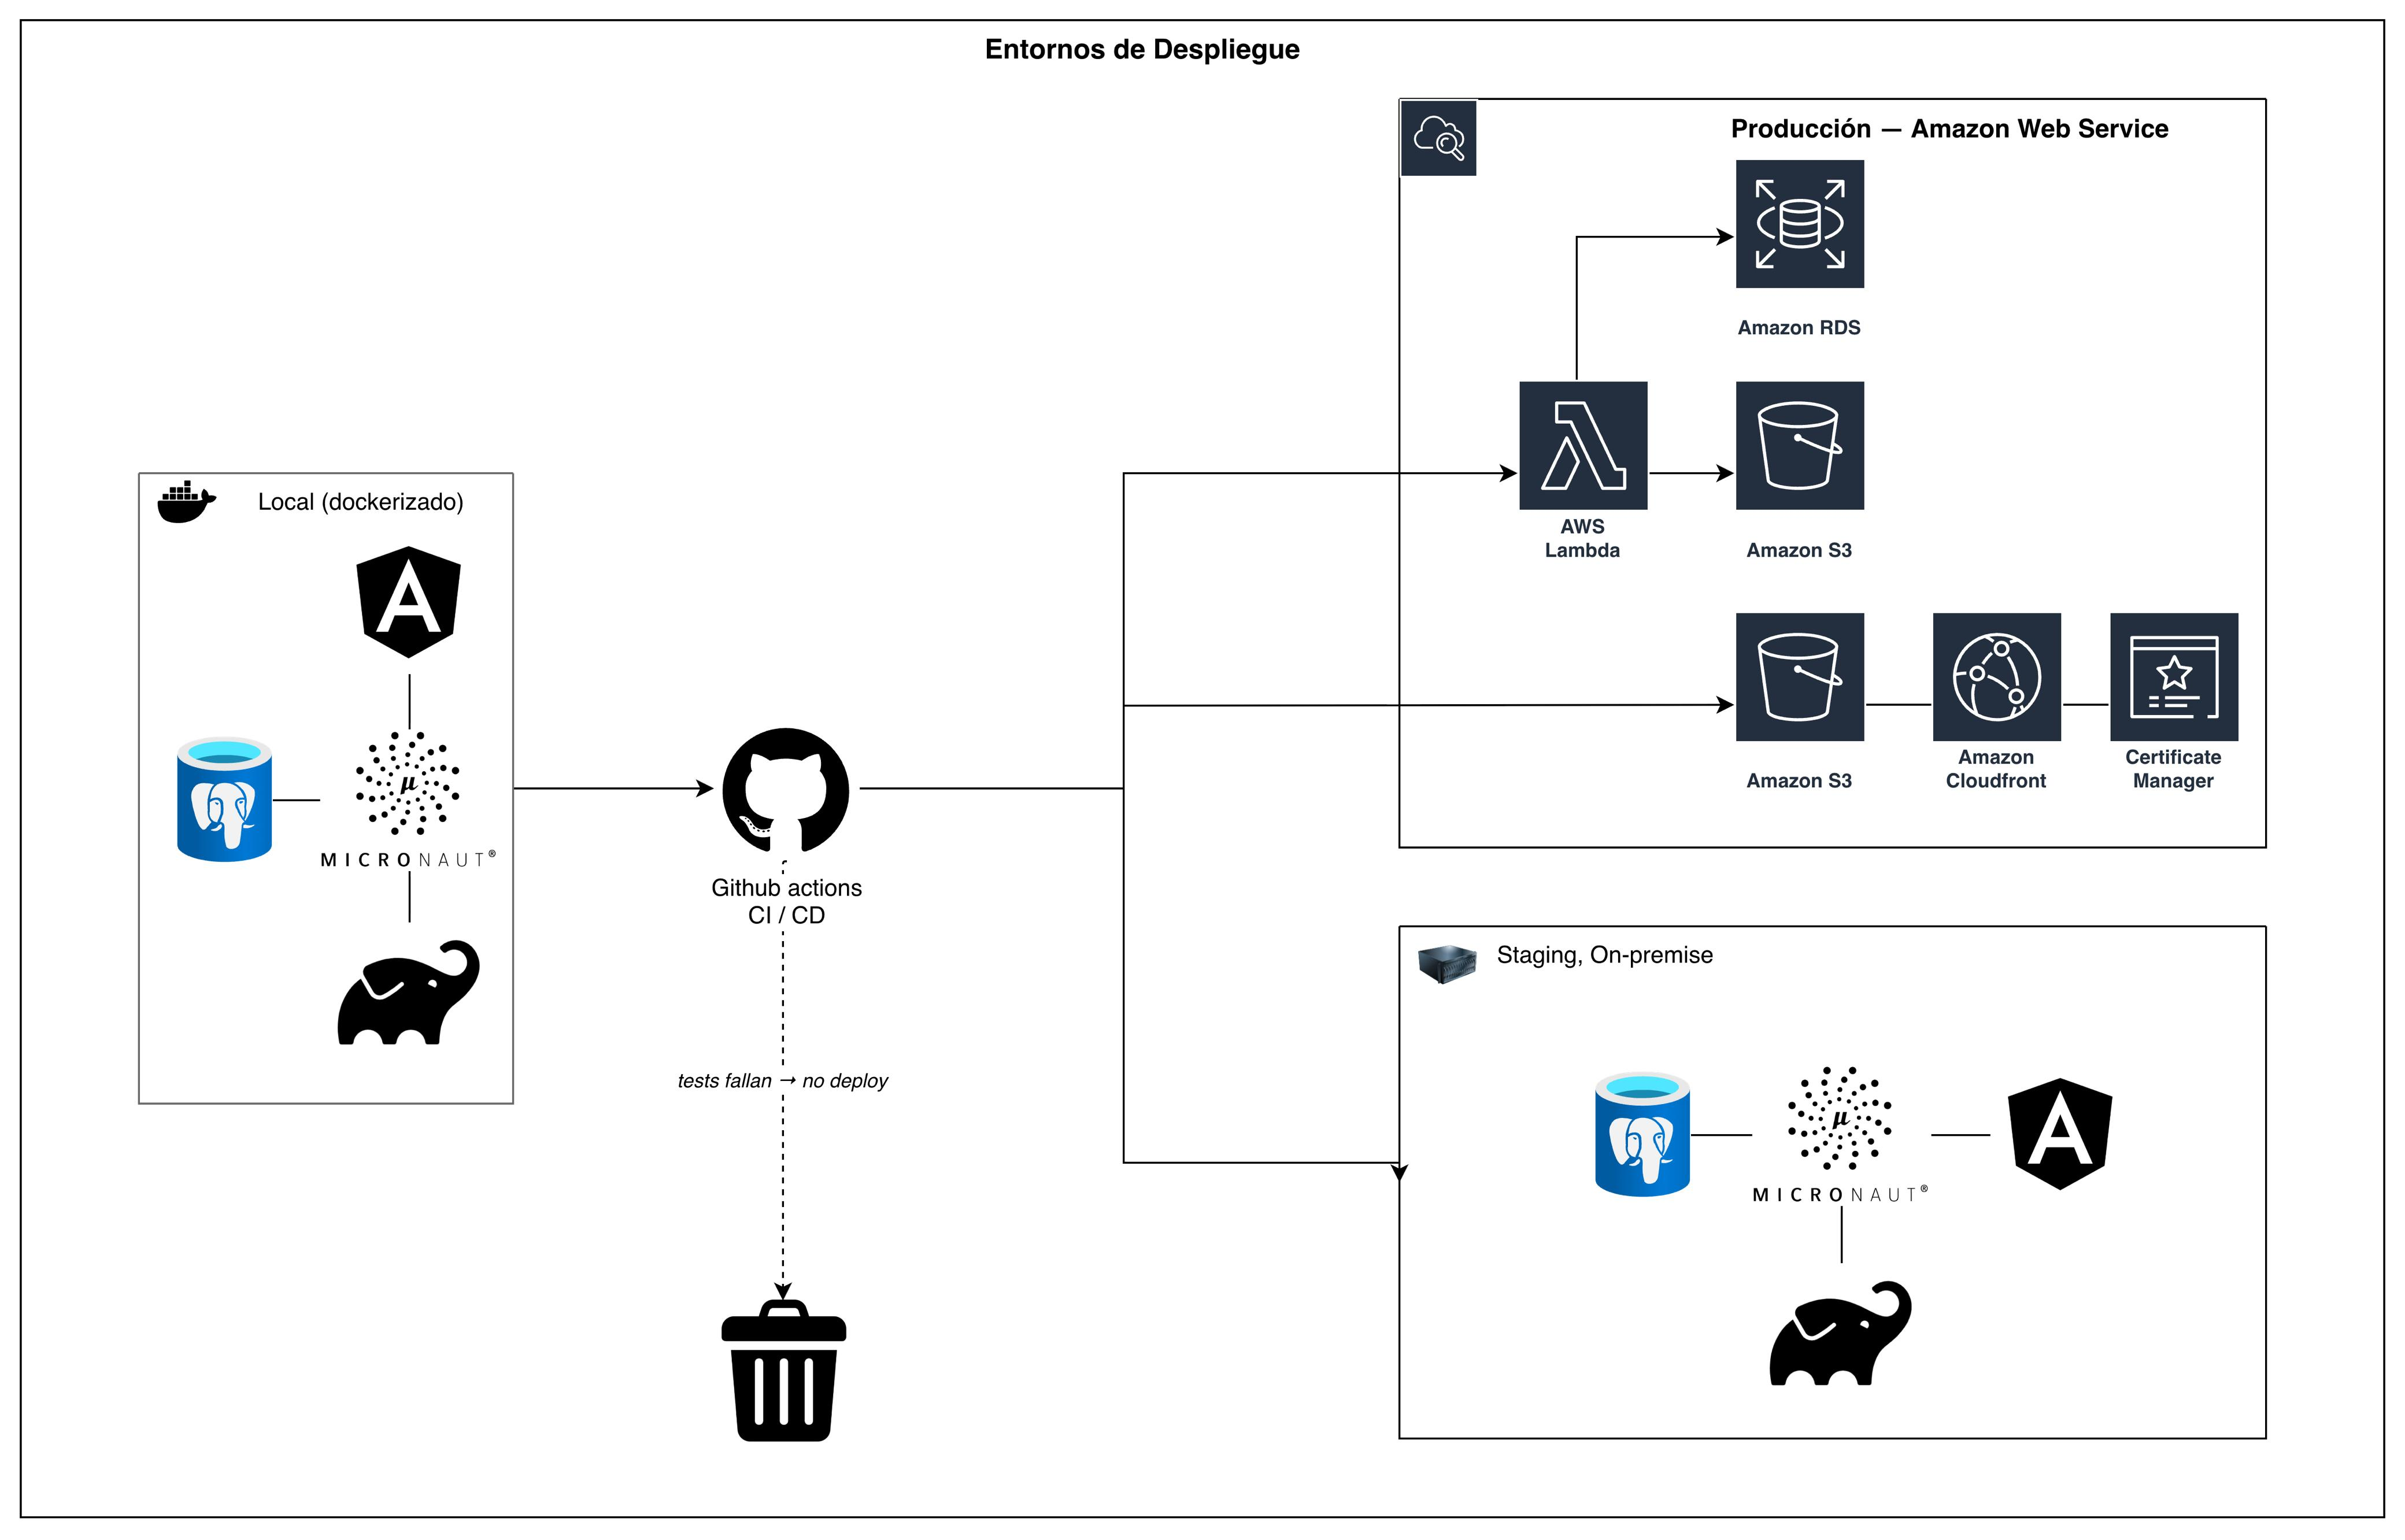
\includegraphics[width=0.95\textwidth]{images/C8/entorno_eco.jpeg}
    \caption{Arquitectura de entornos: desarrollo local, pruebas \textit{on-premise} y orquestación hacia producción.}
    \label{fig:entornos-despliegue}
\end{figure}